\documentclass[tikz,border=10pt]{standalone}
\begin{document}

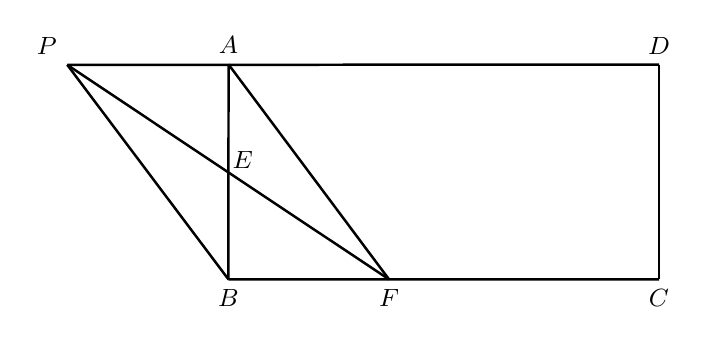
\begin{tikzpicture}[line width=0.9pt, line join=round]
\coordinate (A) at (-1.848,1.373);
\coordinate (B) at (-1.849,-1.357);
\coordinate (C) at (3.619,-1.358);
\coordinate (D) at (3.619,1.370);
\coordinate (F) at (0.191,-1.358);
\coordinate (P) at (-3.896,1.367);


\coordinate (E) at (-1.848,0.000);


\draw (P) -- (D);
\draw (D) -- (C);
\draw (B) -- (F) -- (C);
\draw (A) -- (B);
\draw (P) -- (B);
\draw (P) -- (E) -- (F);
\draw (A) -- (F);


\node[above left]  at (P) {\fontsize{9}{10.8}\selectfont $P$};
\node[above]       at (A) {\fontsize{9}{10.8}\selectfont $A$};
\node[above]       at (D) {\fontsize{9}{10.8}\selectfont $D$};
\node[below]       at (B) {\fontsize{9}{10.8}\selectfont $B$};
\node[below]       at (F) {\fontsize{9}{10.8}\selectfont $F$};
\node[below]       at (C) {\fontsize{9}{10.8}\selectfont $C$};
\node[above right, inner sep=1pt] at (E) {\fontsize{9}{10.8}\selectfont $E$};
\end{tikzpicture}
\end{document}